% Section 4 (Results) of "Conglomerate Mergers under Multiplicative Growth".
% 14 Nov 2026: de-numbered draft. Each paragraph states the claim and anchors it with at most one or two numbers
% (Laplace shocks at alpha = 0.3 as the reference cell); the full cells are in the figures, the two main-text tables
% and the appendix. Simon writes the final prose over this.
% Labels this file expects elsewhere in the paper:
%   sec:Background, sec:Model, sec:Discussion  (existing)
%   sec:growth, sec:conglomerates, sec:decision, sec:calibration  (on the 3.1-3.4 subsections)
%   appendix.tex: app:kstar, app:burnin, app:scope, app:A6, app:rule, app:owners, app:eventstudy, app:burstiness,
%   app:growth, app:A17, app:accept, app:alpha, app:robustness, app:cost, app:nu, app:equalsplit, tab:* and fig:growth_density
% Figures: latex/figures/fig1_scope.tex ... fig6_consent.tex (paper_figures.py), all six placed in this section; tables: latex/tables/*.tex (paper_tables.py).
\section{Results}
\label{sec:Results}

Unless stated otherwise, every number below is from the main block under the power-law cost and the moment rule, the median over five replications, and the reference cell is Laplace shocks at $\alpha = 0.3$. Figures~\ref{fig:scope}--\ref{fig:consent} carry the full grid; Tables~\ref{tab:decomposition} and \ref{tab:owner} the two results the argument rests on; Appendix~\ref{app:results} everything else.

\subsection{The unaffiliated economy}\label{sec:results-baseline}

At $\alpha = 0$ no proposal passes the consent test and the economy is one of 2,500 unaffiliated firms. Its size distribution has the tail that \textcite{axtell2001zipf} documents for US firms, by calibration: the Hill exponent of within-market shares is within 0.06 of the target of 1.06 in every family (Section~\ref{sec:calibration}), and it is the floor that sets it (Appendix~\ref{app:robustness}). The search process runs at the same rate as in every other scenario and none of its proposals is accepted, so the comparison between zero and positive sharing holds the opportunity process fixed and varies only the contract.

Entry is frequent. A standalone firm is recapitalized at minimum scale roughly once every eight to eleven periods, more often the heavier the tails; in the reference cell it hits the floor in 12\% of firm-periods. This rate is the hazard that pooling will be measured against.

\subsection{Scope: why conglomerates stay small}\label{sec:results-scope}

At any positive sharing rate conglomerates form at once and come to hold most of the economy's capital, but they stay small (Figure~\ref{fig:scope}). Scope rises monotonically in $\alpha$, roughly a fifth more members for every tenth of the sharing rate, and stays far below the equal-members reference $K^*$: a third of it in the reference cell, under half under normal shocks and a tenth under $t_3$, where the reference sits at the cap of $M = 50$ markets. The ordering across families is the result to explain. The reference rises steeply with the weight of the tails, because that is where the volatility premium to be recovered is largest, while the scope that forms falls with it, because heavier tails raise the rate at which members are lost to the floor and lower what a window of returns can verify. Pairs are accepted whenever proposed, and acceptance is higher the heavier the tails; what firms refuse is the next member once a unit exists, and that refusal, not the environment, is where most of the distance lies.

\begin{figure}[htbp]
\centering
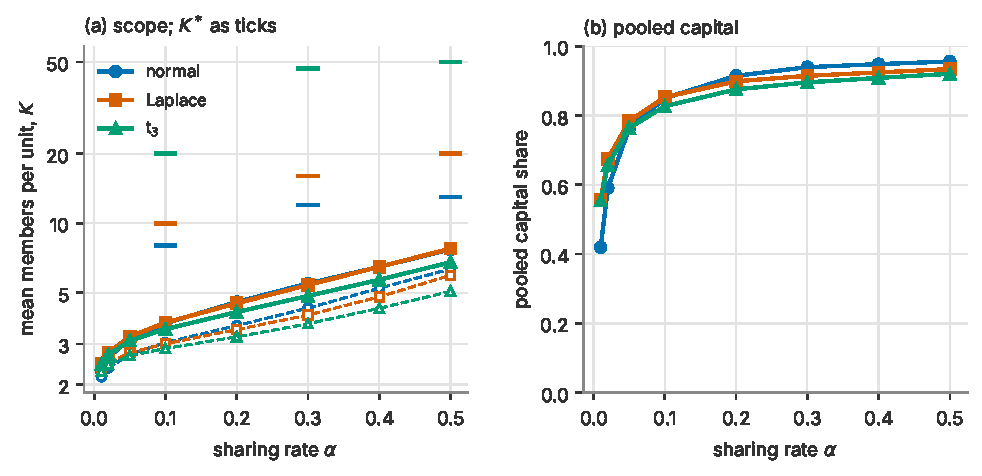
\includegraphics[width=\linewidth]{figures/paper/fig1_scope.pdf}
\caption{Scope and pooled capital by sharing rate. (a) Mean members per unit $K$ against $\alpha$, one line per family, with the loggain rule as a dashed twin and the equal-members reference $K^*$ at $\alpha \in \{0.1, 0.3, 0.5\}$ as ticks; (b) pooled capital share against $\alpha$. Main block to $\alpha = 0.5$ and the same scenarios at $\alpha = 0.6$--$0.9$ (the loggain twin exists to $0.5$), power-law cost; medians over five replications.}
\label{fig:scope}
\end{figure}


Costs are not what stops unit growth. At the scope that forms, the coordination cost is one to three per cent of the pooling gain, and by the marginal calculus of Section~\ref{sec:Background} a further member would pay for itself up to roughly three times the scope reached. Raising the cost lowers scope slowly, about 0.6 members per doubling, and at twenty times the calibrated level, where $K^*$ has fallen to where the units already were, the units have moved down with it (Appendix~\ref{app:cost}).

What stops them is consent on members whose gain to the incumbents is too small to be seen (Figure~\ref{fig:consent}). Acceptance falls monotonically with the size of the prospective unit, from every pair to about one proposal in ten for a twelfth member, at the baseline search rate and at $p = 1$ alike. The member who binds is an incumbent, and the recruit on offer is small: half of the proposals to units of four or more bring a standalone just recapitalized at the floor, whose weight in the prospective unit is a fraction of an equal member's. An incumbent's diversification gain from such a recruit is a third of the equal-weight gain of Section~\ref{sec:Background} at $K = 5$ and a quarter at $K = 8$, and net of the marginal cost it reaches zero between the seventh and the tenth member; the binding member's estimated gain, the smallest over $K$ noisy estimates, crosses zero two members earlier (Appendix~\ref{app:A6}). Firms are not reluctant to pool: they accept every pair, and more of everything under heavier tails. They decline recruits that bring the unit nothing, and the recruits that a floored economy supplies bring little. The one other kind of proposal, the merger of two existing units, fails for the other reason Section~\ref{sec:decision} allows: when the two units differ in volatility, pooling moves arithmetic growth from the volatile unit to the calm one, and it is the volatile unit's members whose consent fails. The loggain rule, which estimates the same gain by a replayed sample mean, sees less again and forms units one to two members smaller, because on a window of fifty periods its estimate is both noisier and biased low; an exact replay with that bias removed behaves like the moment rule (Appendix~\ref{app:rule}).

\begin{figure}[htbp]
\centering
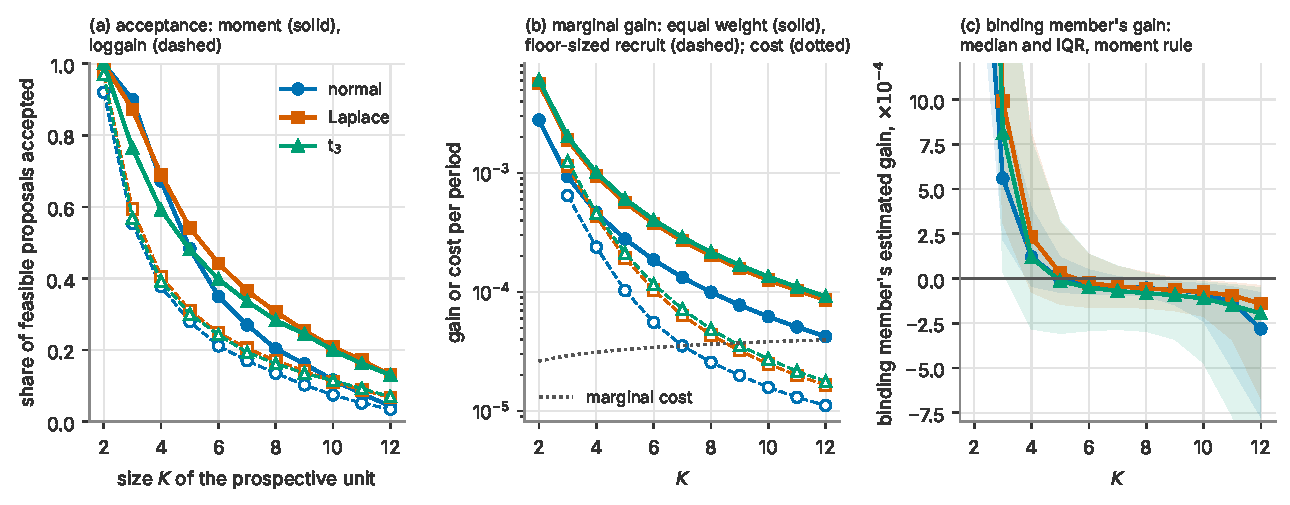
\includegraphics[width=\linewidth]{figures/paper/fig6_consent.pdf}
\caption{Consent by scope. (a) Acceptance rate by size $K$ of the prospective unit at $\alpha = 0.3$ under the moment and loggain rules ($p = 0.05$ and $p = 1$); (b) the equal-weight marginal gain of the $K$-th member, the incumbents' gain from a floor-sized recruit and the marginal cost, log axis; (c) the binding member's estimated gain by $K$ (median and IQR).}
\label{fig:consent}
\end{figure}


The window is the direct test of this bound. Memory lengthens scope slowly and without saturation (Figure~\ref{fig:search}c): a longer window shrinks the sampling error of the second moments and lets more marginal members pass, but a twenty-five-fold longer window still leaves scope under half of the reference. Under the moment rule voluntary exits are nil at every window length; under the loggain rule they vanish once the window is long enough, which says that the exits a longer window removed were decisions taken on noise. The exits that remain at every window length are deaths at the floor: the attrition that bounds scope under heavy tails is set by the floor, not by the firms' patience.

\begin{figure}[htbp]
\centering
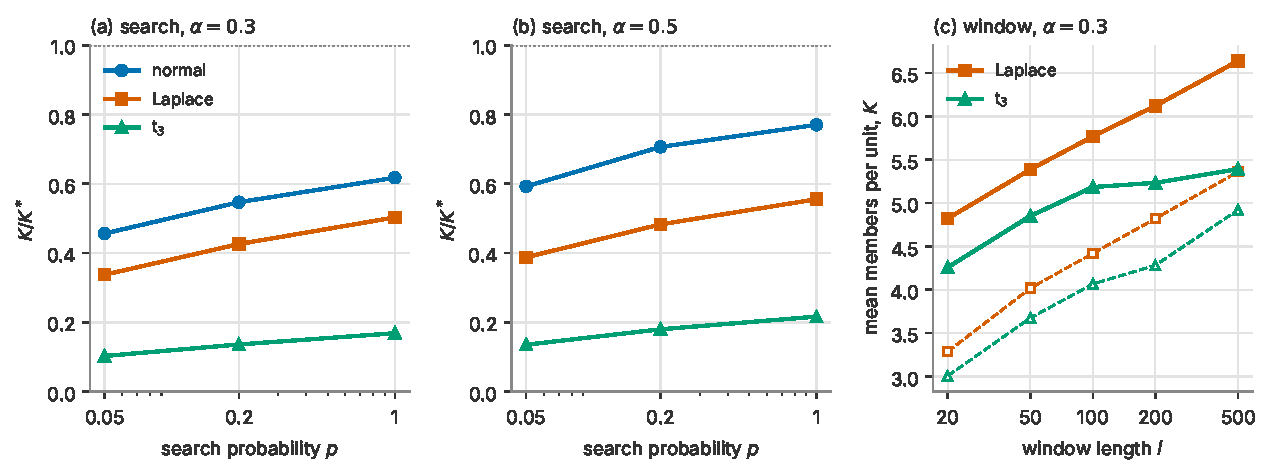
\includegraphics[width=\linewidth]{figures/paper/fig2_search.pdf}
\caption{Scope relative to the equal-members reference, $K/K^*$, against the proposal probability $p \in \{0.05, 0.2, 1\}$ at $\alpha = 0.3$ and $0.5$, one line per family. Search block and main block, power-law cost; medians over five replications.}
\label{fig:search}
\end{figure}


Whether that refusal is a shortfall turns on the capital weights of the members. The equal-members reference assumes every recruit is as large as the incumbents; the recruits that arrive are floor-sized, worth little to the incumbents and worth the whole variance cut and the hazard reduction of Section~\ref{sec:results-owners} to themselves. The contract offers no instrument --- one rate for the whole unit, no side payments --- by which the recruit could pay for admission, so the firms, who know the weights where no formula does, refuse. The distance to $K^*$ is for the most part the distance between a configuration of equal members and the configuration the economy offers; it is not a friction that more search would remove, and the structure that forms is not the one that would be chosen with full information.

Turnover is high: members are ejected at the floor and replaced by mergers at the same rate, so the population of conglomerates is a steady state of churn, and firms with heavier tails are not less willing to pool but less able to stay pooled (Appendix~\ref{app:scope}). But churn is not what sets the level. Table~\ref{tab:decomposition} puts the base case between four other economies that share its seeds. With consent switched off --- a control with no knowledge, not a behavioural alternative --- units are as large as the floor and the one-firm-per-market constraint allow, and under normal and Laplace shocks they are larger than the equal-members reference itself: the environment permits more than the equal-members arithmetic recommends, and the whole distance to the scope that forms is consent. Only under $t_3$ does the control stop short of the reference, so that attrition takes part of the distance. With every market at the same volatility scope barely changes, so the conflict between members of unequal volatility is immaterial at these ranges; with the gain estimated by a sample mean it falls by one to two members, which is verifiability in the strict sense. In the reference cell consent accounts for seven tenths of what the environment permits and verifiability for one tenth. What consent refuses is recruits, not partners: with consent off the extra mergers are almost all solo entries of floor-sized firms, and the extra scope buys the economy little (Appendix~\ref{app:accept}). Scope is bounded by consent first and by what a window can verify second; attrition binds only under heavy tails; and cost is the margin that would bind only in a calmer economy.

\begin{table}[htbp]
\centering
\caption{Scope under five rules and the two differences that bound it, power-law cost; medians over five replications}
\label{tab:decomposition}
\small
\begin{tabular}{lrrrrrrrr}
\toprule
Family & $\alpha$ & $K^*$ & $K_{\text{accept}}$ & $K_{\text{hom}}$ & $K$ & $K_{\text{loggain}}$ & Consent & Verif. \\
\midrule
normal & 0.1 & 8 & 17.6 & 3.8 & 3.7 & 3.0 & 13.9 (79\%) & 0.6 (4\%) \\
 & 0.3 & 12 & 22.2 & 5.6 & 5.5 & 4.3 & 16.8 (75\%) & 1.2 (5\%) \\
 & 0.5 & 13 & 28.2 & 8.0 & 7.7 & 6.3 & 20.5 (73\%) & 1.4 (5\%) \\
\midrule
Laplace & 0.1 & 10 & 13.8 & 3.8 & 3.7 & 3.0 & 10.1 (73\%) & 0.7 (5\%) \\
 & 0.3 & 16 & 18.1 & 5.5 & 5.4 & 4.0 & 12.7 (70\%) & 1.4 (8\%) \\
 & 0.5 & 20 & 24.3 & 8.2 & 7.8 & 5.9 & 16.5 (68\%) & 1.8 (7\%) \\
\midrule
$t_3$ & 0.1 & 20 & 12.4 & 3.5 & 3.5 & 2.9 & 8.9 (72\%) & 0.6 (5\%) \\
 & 0.3 & 47 & 16.2 & 4.9 & 4.8 & 3.7 & 11.4 (70\%) & 1.2 (7\%) \\
 & 0.5 & 50 & 21.8 & 7.0 & 6.8 & 5.1 & 15.0 (69\%) & 1.7 (8\%) \\
\bottomrule
\end{tabular}
\par\smallskip\begin{minipage}{0.95\linewidth}\footnotesize $K^*$: equal-members reference (Section 3.4). $K_{\text{accept}}$: every feasible proposal accepted and no voluntary exit, i.e. the scope the floor and the one-firm-per-market constraint alone permit (a control without knowledge). $K_{\text{hom}}$: homogeneous economy (every market at $q = 0.20$), moment rule. $K$: base case. $K_{\text{loggain}}$: the same gain estimated by its sample mean. Consent $= K_{\text{accept}} - K$, Verif.\ (verifiability) $= K - K_{\text{loggain}}$; shares of $K_{\text{accept}}$ in parentheses. The transfer conflict between members of unequal volatility, $K_{\text{hom}} - K$, is 0.0--0.4 members in every cell (at most 4\% of $K^* - K_{\text{loggain}}$) and is not shown.\end{minipage}
\end{table}


Raising the rate at which members are found raises scope with diminishing returns (Figure~\ref{fig:search}a,b): when every firm proposes every period, mergers and floor exits triple together, acceptance falls, and scope rises by a third to two thirds, stopping at half of the reference in the reference cell and a sixth under $t_3$. With search unlimited the firms exhaust what the recruits on offer are worth to the unit; what remains is the distance between a configuration of equal members and the one the economy offers. Under heavy tails the unit cannot retain members fast enough, and $t_3$ is exactly where $K^*$ is largest: the firm that would gain most from pooling is the one least able to stay pooled.

\subsection{Owners' growth and survival}\label{sec:results-owners}

The results so far are about structure; this one is about what membership is worth to the firm's owners, measured directly. For the 27 traced runs we observe every firm in every post-burn-in period and compare the next-period owner return --- the log change in the firm's share net of any floor recapitalization, which is capital the owners did not earn --- of members and standalones in the same market and the same size decile, with affiliation taken at the start of the period. The comparison is within market and within size, so it does not reward members for being in calmer markets or for being large. Nor does it reward them for having passed the consent test: shocks are independent across periods, so a firm's next-period return does not depend on the window that admitted it, only on its market, its size through the floor, and whether it is pooled. The gain is a gain in the firm's share of its market, and since market capital is fixed it is, within each market, the co-market standalones' loss; what pooling adds to the economy is in Section~\ref{sec:results-distribution}.

The member--standalone gap in mean owner return is positive in every cell and every replication (Figure~\ref{fig:owner_return}, Table~\ref{tab:owner}): 0.85 percentage points per period in the reference cell. It is close to linear in $\alpha$, largest in the largest units, flat across size deciles except for a dip in the largest, and ordered $t_3 >$ Laplace $>$ normal, as the volatility premium $\tfrac12\alpha(2-\alpha)\sigma^2$ of Section~\ref{sec:Background} predicts; part of the $t_3$ gain is the diversification of the within-market factor $G$ that no firm can escape by staying put. The loggain rule's smaller units gain a little less.

\begin{table}[htbp]
\centering
\caption{Owners' time-average growth and ruin hazard by affiliation status}
\label{tab:owner}
\small
\begin{tabular}{lrrrrr}
\toprule
Family & $\alpha$ & Gap, mean & Gap, median & Ordinary share & Hazard ratio \\
\midrule
normal & 0.05 & 0.07 & 0.02 & -0.20 & 10.6 \\
 & 0.1 & 0.16 & 0.06 & 0.22 & 12.0 \\
 & 0.3 & 0.51 & 0.32 & 0.50 & 18.2 \\
\midrule
Laplace & 0.05 & 0.10 & 0.01 & -0.50 & 8.5 \\
 & 0.1 & 0.26 & 0.11 & 0.03 & 9.5 \\
 & 0.3 & 0.85 & 0.41 & 0.38 & 13.9 \\
\midrule
$t_3$ & 0.05 & 0.27 & 0.01 & -0.24 & 7.4 \\
 & 0.1 & 0.48 & 0.10 & -0.03 & 8.3 \\
 & 0.3 & 1.19 & 0.40 & 0.22 & 11.7 \\
\bottomrule
\end{tabular}
\par\smallskip\begin{minipage}{0.95\linewidth}\footnotesize Owner return: next-period log change of the firm's market share net of floor recapitalization; gap = member $-$ standalone within market $\times$ size decile, in percentage points per period; 27 traced runs, means over three replications. Ordinary: share of the mean gap accruing in periods without a floor hit. Hazard ratio: floor hits per standalone-period over floor hits per member-period, same cells (Table~\ref{tab:hazard}).\end{minipage}
\end{table}

\begin{figure}[htbp]
\centering
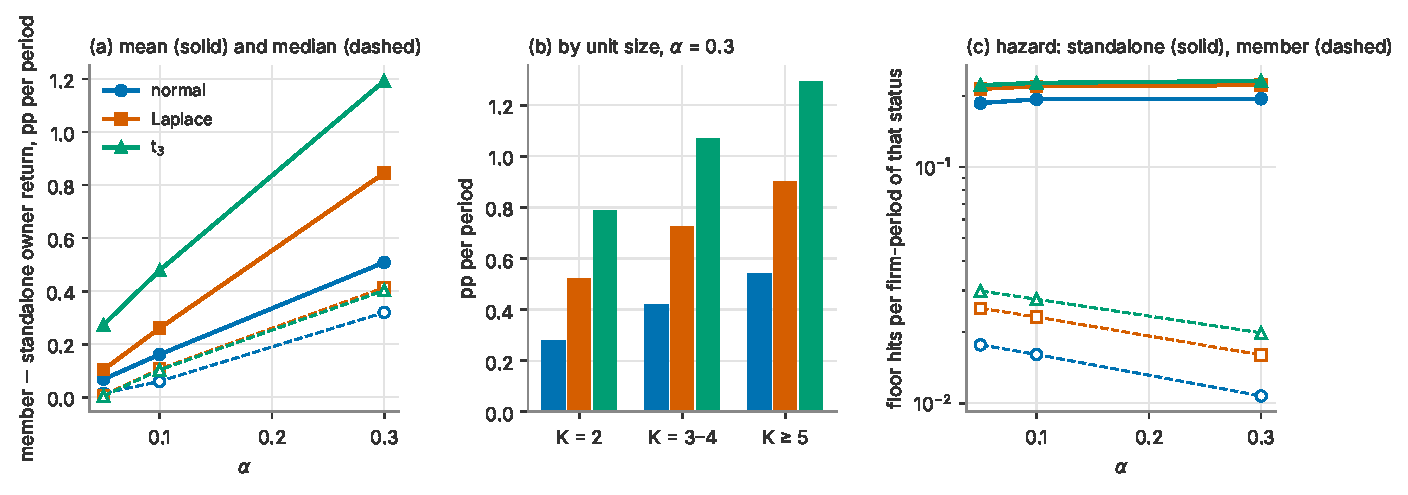
\includegraphics[width=\linewidth]{figures/paper/fig3_owner_return.pdf}
\caption{Member--standalone owner-return gap. (a) Mean (solid) and median (dashed) gap by family and $\alpha$, percentage points per period; (b) the gap by unit size ($K = 2$, 3--4, $5+$) at $\alpha = 0.3$; (c) floor hits per firm-period by status (standalone solid, member dashed). The 27 traced runs.}
\label{fig:owner_return}
\end{figure}


The gain is partly ordinary growth and partly avoided ruin, in proportions set by the tails. Splitting the firm-periods by whether the firm reaches the floor in the next period, an exact accounting of the gap, the ordinary-period part is half of the gain under normal shocks and a fifth under $t_3$ (Table~\ref{tab:owner}); in those periods a member's owners grow faster than a standalone's in the same market and size decile by the volatility drag of Section~\ref{sec:growth} that pooling removes. The remainder is that members reach the floor less often and lose less when they do: pooling cuts the hazard by a factor of seven to eighteen, more at higher $\alpha$ (Appendix~\ref{app:owners}). At low sharing rates the ordinary-period part is nil and the whole gain is ruin protection, which is where the median loses sight of the mean: the median gap is a third to three fifths of the mean, and at $\alpha = 0.05$ it is indistinguishable from zero while the mean is clearly positive, because the benefit of pooling lives in the catastrophic periods that a typical window does not contain. An institution whose value is avoided catastrophe is undervalued by any evaluation of typical periods, and most by the firms that need it most.

\subsection{The sharing rate firms choose}\label{sec:results-alpha}

The sharing rate has so far been imposed. When units set it themselves --- every period, by unanimity, on the demeaned window --- they choose to pool nearly everything they earn: starting from $\alpha = 0.1$, the adopted rate averages 0.9 in every family, is never zero and is one in a sizeable minority of unit-periods (Figure~\ref{fig:hill}, Appendix~\ref{app:alpha}). Read as an internal capital market, it is the share of operating cash flow that passes through headquarters and is reallocated across divisions rather than retained where it was earned \citep{stein1997internal, lamont1997cash}. With members of equal volatility the gain of Section~\ref{sec:Background} increases in $\alpha$ throughout, so a symmetric unit would pool fully; that units stop short of one is the mark of unanimity among unequal members, since a member whose volatility is below the unit's has less to gain from a higher rate and can veto it. Neither the dispersion of members' volatilities nor their level drives the choice. The scope these units reach, three times that of the $\alpha = 0.3$ cell, is what the rate implies rather than a separate effect: a fixed $\alpha = 0.9$ reproduces the block, so renegotiation itself adds little, and the finding of the block is the rate.

\begin{figure}[htbp]
\centering
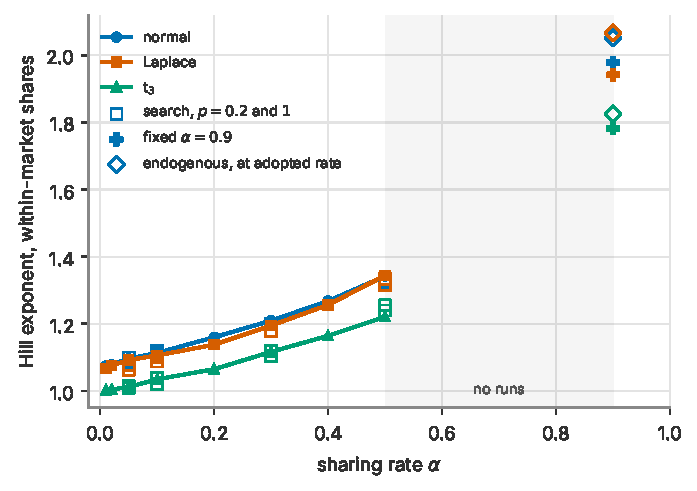
\includegraphics[width=\linewidth]{figures/paper/fig4_hill_alpha.pdf}
\caption{Tail exponent against the sharing rate. Hill exponent of within-market shares: main-block medians as lines by family; the $\alpha = 0.9$ cell and the search, lookback, correlation and homogeneous blocks as markers; the endogenous block at its adopted rate. The exponent rises with $\alpha$, by about 0.45 per unit up to 0.5 and faster beyond, and does not respond to scope or to the number of firms pooling.}
\label{fig:hill}
\end{figure}


\subsection{Mechanisms: contract terms before environment}\label{sec:results-mechanisms}

One block varies the terms on which firms pool rather than the environment they pool in, and the sharing rule decides whether conglomerates exist at all. Under equal dollar splits of the net pool, scope stays at two to three members at every sharing rate and pooled capital never exceeds a third of the economy, against up to 96\% under proportional sharing (Appendix~\ref{app:equalsplit}). Under an equal split the larger partner subsidizes the smaller in every period in which it does better, which it expects to do half the time, and refuses; the units that do form shed members by choice every period, where proportional units shed none. The occasional ruin of a small member under equal sharing, charged to its partners, is not what holds scope down; refusal is. The other contract term, the length of memory, is in Section~\ref{sec:results-scope}, where it belongs to the verifiability bound.

\subsection{What pooling does to the size distribution}\label{sec:results-distribution}

The tail exponent rises with the sharing rate, and with nothing else (Figure~\ref{fig:hill}): from its calibrated value near 1.06 at $\alpha = 0$ to 1.2 in the reference cell and to about 2 at $\alpha = 0.9$, where units that set their own rate also sit. The rise is convex, about 0.45 per unit of $\alpha$ up to $0.5$ and 1.5 per unit beyond, in every family. Scope and the number of firms pooling do not enter: the search block triples mergers and raises scope by a third to two thirds at the same rate without moving the exponent. Pooling thins the upper tail by the mechanism of Section~\ref{sec:growth}. Every firm loses share to its market on average, by Jensen's inequality; a member loses it at $(1-\alpha)$ times the standalone rate, which is the owner-return gain of Section~\ref{sec:results-owners}, so a member's expected growth is higher, not lower. What thins the tail is the compression of realized factors within a period: a member's lucky draw is shared with its partners and their unlucky draws with it, so the runs of large draws that carry a firm into the upper tail are rarer among members. Less dispersion of growth across firms in each period, and a higher time average for each firm across periods, are the same fact seen from two sides; it is the volatility tax that falls, not the firm's growth. The compression is visible in the members' own growth rates (Appendix~\ref{app:growth}): their dispersion is what pooling gross returns at the units' actual weights predicts, and the cut falls on the lower tail, because a large own loss is floored by the partners' share while a large own gain passes through. Pooling rescales a member's growth-rate distribution and trims its lower tail but leaves its family unchanged: Laplace members are still Laplace, normal members still normal, and $t_3$ members still heavier-tailed than either. Within markets firms thereby become more equal: the within-market Herfindahl index falls with $\alpha$ in every family. The share of the economy's capital held by the largest tenth of owning units, a conglomerate counted as one owner, rises moderately with $\alpha$ under heavier tails and not at all under normal shocks up to $\alpha = 0.5$; beyond that it falls under normal and Laplace shocks as units grow more equal in size, and only under $t_3$ does it keep rising (Appendix~\ref{app:A17}). Neither measure speaks to competition in a product market: a unit holds one firm per market, so horizontal concentration is excluded by construction, and what pooling concentrates is the ownership of capital across markets, not supply within any one.

Compression of sizes is not mobility of ranks. Pooling lowers rank mobility within markets rather than raising it, partly because fewer firms are recapitalized at the floor and partly because members' ranks move less than standalones' among going concerns, and it makes the top decile of owning units markedly more persistent, keeping two thirds of its membership over 100 periods against a third to a half without pooling (Appendix~\ref{app:A17}). Pooling thus makes the size distribution within markets more equal and its ranks stickier, and makes the largest owners both somewhat larger and markedly more persistent.

Exits from conglomerates happen in bursts, which pooling damps considerably (Figure~\ref{fig:burstiness}). Floor hits within a market-period are overdispersed, three to five times the binomial reference, and the worst market-period in a run sees nearly every firm in the market at the floor at once. The source is the cross-sectional factor $G$ of Section~\ref{sec:growth}: one firm's large draw lowers every other firm's relative return in its market. The index falls with $\alpha$ in every family because members absorb part of the burst with capital from other markets.

\begin{figure}[htbp]
\centering
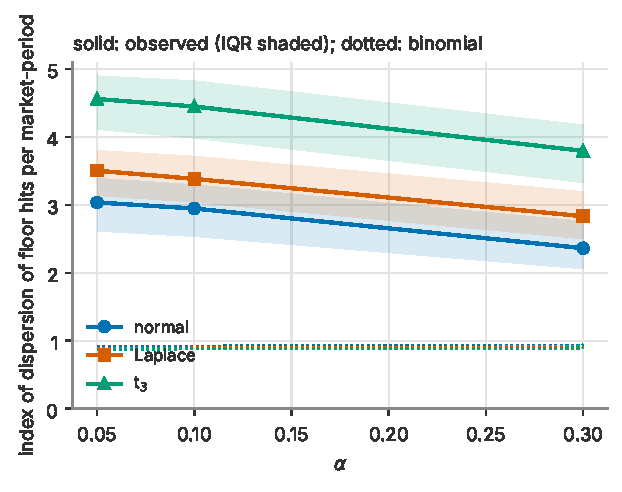
\includegraphics[width=\linewidth]{figures/paper/fig5_burstiness.pdf}
\caption{Clustering of floor hits. Index of dispersion of floor hits per market-period by family and $\alpha$ (median and IQR over the traced replications) against the binomial reference.}
\label{fig:burstiness}
\end{figure}


\subsection{Robustness}\label{sec:results-robustness}

Appendix~\ref{app:robustness} gives every block in full and Tables~\ref{tab:robustness} and \ref{tab:robustness-b} summarize them. The cost form moves scope by under one member at equal $\Phi(40)$ and the level by about 0.6 members per doubling; cross-market correlation of 0.3 leaves scope within 0.2 of the baseline; the floor level sets the tail and little else; economy size matters only through the number of firms per market, with the floor recalibrated to each $N$. Heavier tails than $t_3$ lower scope through attrition, not consent: at $\nu = 2.5$ acceptance is higher than at $\nu = 4$ and scope lower, because floor exits rise faster than acceptance. Burn-in is checked by extending the headline cells to 16,000 periods (Appendix~\ref{app:burnin}). The appendix also reports, from the same traces, the growth of joiners against same-market standalones after entry; it is positive in every cell but is not a clean counterfactual, for a reason given there, and the owner-return result rests on the status panel alone (Appendix~\ref{app:eventstudy}).

% ---------------------------------------------------------------------------
% Hand-over material from the Section 4 doc (not paper text): the doc's header, the "Appendix material" passages cut
% from the main text (for the appendix tex), Table 6b's content, and the exhibit specification. Kept here so nothing is lost.
\iffalse
# Section 4 draft — Results

Nov 4, 2026 · @Simon

## How to read this draft

Settled Section 4 text for the writing pass (13 Nov). Every number is recomputed from the pilot D files at the referee-fixes tip (cd6dc76); unless stated otherwise: main block, power-law cost, proportional sharing, moment decision rule; K is the mean number of members per unit over active units and post-burn-in snapshots, medians across the five replications; α = 0.3 is the reference cell; the loggain rule (pilot C, same seeds) is quoted beside the base case as “loggain: …”. Tables are generated in latex/tables (analysis/paper\\_tables.py) and figures in figures/paper (analysis/paper\\_figures.py); the exhibit list and the “Appendix material” section below are hand-over material for the tex transfer.

## Appendix material (moved out of the main text in the cut pass, unchanged)

The effective number of members is smaller still: K\\_eff/K, the inverse Herfindahl of members' weights over K, is 0.68–0.70 at α = 0.3, so the typical unit is a few partners of unequal size rather than an equal-weighted pool.

Units that choose their rate reach 16.9 (normal), 18.0 (Laplace) and 14.3 (t₃) mean members under the power-law cost, with 95–98% of capital pooled and a tail exponent of 1.8–2.1. This is the scope that a rate of 0.9 implies, not a separate effect: along the fixed-rate grid K rises from 5.4 at α = 0.3 to 7.8 at 0.5, and the grid stops there. The finding of the block is the rate. The ordering across families is the same as before: the heaviest tails choose a slightly lower rate and reach a smaller scope. The exponential-cost cells reach K = 16–23 at a lower pooled share (81–92%), because that form charges small units most.

Neither heterogeneity among members nor the volatility of their markets drives the choice. Across 7,630 units active at the end of a run, the Spearman correlation of a unit's time-averaged rate with the dispersion of its members' volatilities is −0.14 to 0.00, and with their mean volatility 0.04–0.10. Under the loggain rule the latter was 0.14–0.26: units in more volatile markets pooled more, not because the optimum differed — it is full pooling at every volatility level — but because only there was the gain from a higher rate large enough to show through the window's noise. With the second-moment estimator it shows everywhere, and the choice is nearly uniform.

Under equal dollar splits of the net pool (normal shocks, all four cost forms), mean scope is 2.1–3.2 at every sharing rate from 0.01 to 0.5 and pooled capital never exceeds 34%, against 3.2–7.7 and up to 96% under proportional sharing. The reason is visible in who consents. Proposals between two unaffiliated firms pass at 3–48% under equal sharing against 95–100% under proportional; proposals of a standalone to a unit pass at 6–17% against 28–41%. Under an equal split the larger partner subsidizes the smaller in every period in which it does better, which it expects to do half the time, and refuses; and the units that do form shed two to five members per period by choice, where proportional units shed none, because the exit test now detects the loss. The occasional ruin of a small member under equal sharing (0.01–0.05 members per period at α ≥ 0.3, charged to its partners) is not what holds scope at two or three; refusal is.

Within markets firms become more equal; across the economy the units that own them become fewer and larger. The within-market Herfindahl index falls from 0.175–0.20 at α = 0 to 0.14–0.17 at α = 0.3 and 0.11–0.14 at α = 0.5. The capital held by the largest ten per cent of units — a conglomerate counted as one owner — goes the other way, from 0.65 to 0.65 (normal, with 0.67 at α = 0.3), 0.66 to 0.74 (Laplace) and 0.68 to 0.79 (t₃) between α = 0 and 0.5. Whether pooling concentrates or deconcentrates depends on the question: it deconcentrates each market and concentrates ownership, and the two measures answer different questions. Horizontal effects are excluded by construction, since no unit holds two firms in one market.

Units sort by volatility and grow unequal. Assortativity — the dispersion of members' market volatilities relative to that of a random set of the same size — falls from 0.60–0.61 at α = 0.01 to 0.35–0.36 at α = 0.5: members are more alike in volatility than chance, and increasingly so, because the consent test selects partners whose fluctuations are worth sharing from both sides. Within the unit, the effective number of members K\\_eff/K falls from 0.83–0.88 to 0.64–0.68 over the same range as units accumulate a few large members and many recruits from the floor.

Table 6b — Cost level, power-law form, α = 0.3, moment rule (K loggain beside); medians over five replications (×0.5 and ×2 from the cost-level block, Laplace only; ×5–×20 from the cost-level-high block)

| Family | × cost level | K | K, loggain | K\\* | K/K\\* | Pooled capital | Acceptance | Hill |
| --- | --- | --- | --- | --- | --- | --- | --- | --- |
| Laplace | 0.5 | 6.0 | 4.3 | — | — | 0.92 | 0.42 | 1.20 |
| Laplace | 1 | 5.4 | 4.0 | 16 | 0.34 | 0.91 | 0.40 | 1.19 |
| Laplace | 2 | 4.7 | 3.7 | — | — | 0.91 | 0.36 | 1.19 |
| Laplace | 5 | 3.9 | 3.1 | 8 | 0.49 | 0.87 | 0.31 | 1.17 |
| Laplace | 10 | 3.3 | 2.8 | 6 | 0.55 | 0.79 | 0.29 | 1.15 |
| Laplace | 20 | 2.8 | 2.5 | 4 | 0.70 | 0.67 | 0.29 | 1.13 |
| t₃ | 1 | 4.8 | 3.7 | 47 | 0.10 | 0.90 | 0.44 | 1.12 |
| t₃ | 5 | 3.7 | 3.0 | 10 | 0.37 | 0.86 | 0.38 | 1.10 |
| t₃ | 10 | 3.3 | 2.8 | 7 | 0.47 | 0.80 | 0.37 | 1.07 |
| t₃ | 20 | 2.8 | 2.5 | 5 | 0.57 | 0.70 | 0.36 | 1.05 |

## Figures and tables (specification for `analysis/paper_figures.py`)

| Exhibit | Content | Source columns (pilot\\_d unless stated) |
| --- | --- | --- |
| Figure 1 | Scope K versus α, one line per family, loggain as dashed twin, K\\* at α ∈ {0.1, 0.3, 0.5} as markers; second panel pooled capital share versus α | tidy.csv main/power\\_law: K\\_mean, cong\\_capital\\_share\\_median (median over reps); pilot\\_c/tidy.csv for the loggain twin; benchmarks.csv K\\_star |
| Figure 2 | (appendix) K/K\\* versus search probability p ∈ {0.05, 0.2, 1} at α = 0.3 and 0.5, one line per family; three points, no fitted curve | tidy.csv search + main/power\\_law: K\\_mean; benchmarks.csv |
| Figure 3 | Member–standalone owner-return gap: panel (a) mean and median by family and α; panel (b) by scope (K = 2, 3–4, 5+); panel (c) floor-hit rate per status | status\\_panel\\_summary.csv: diff\\_fe\\_mean, diff\\_fe\\_median, diff\\_K2\\_mean, diff\\_K3\\_4\\_mean, diff\\_K5p\\_mean, floor\\_rate\\_member, floor\\_rate\\_standalone |
| Figure 4 | (appendix) Hill exponent versus the sharing rate α: main-block medians as lines by family, the α = 0.9 cell and the search, lookback, correlation and homogeneous blocks as markers, the endogenous block at its adopted rate. Caption: the exponent rises with α (about 0.45 per unit up to 0.5, faster beyond) and does not respond to scope or to the number of firms pooling. figures/paper/fig4\\_hill\\_alpha. | tidy.csv: hill\\_exponent\\_median against alpha (alpha\\_adopted\\_median for the endogenous block) |
| Figure 5 | (appendix) Floor-hit clustering: index of dispersion by family and α with the binomial reference | burstiness\\_summary.csv: D\\_median, D\\_p25, D\\_p75, D\\_binomial |
| Figure 6 | Consent by scope: acceptance rate by size K of the prospective unit (α = 0.3, p = 0.05 and 1), moment and loggain; marginal gain into K and marginal cost on a log axis; the binding member's estimated gain (median, IQR) by K | acceptance\\_by\\_K.csv: proposals, mergers, acceptance, binding\\_median, binding\\_p25/p75, marginal\\_gain\\_into\\_K, marginal\\_cost\\_into\\_K; pilot\\_c/acceptance\\_by\\_K.csv for loggain |
| Table 3 | K, K loggain, K\\*, K/K\\*, pooled share, floor and voluntary exits per period, acceptance, member and standalone floor-hit rate per status-period; family × α ∈ {0.05, 0.1, 0.3, 0.5} | tidy.csv main/power\\_law (floor\\_hit\\_rate\\_\\*\\_status); pilot\\_c/tidy.csv |
| Table 3b | K by window length, moment / loggain (in the text; the exit rows become a note) | tidy.csv lookback; pilot\\_c/tidy.csv |
| Table 3c | Decomposition of K\\* − K\\_loggain into survival and feasibility, transfer conflict, verifiability; family × α ∈ {0.1, 0.3, 0.5} | consent\\_gap\\_decomposition.csv |
| Table 4 | Owner-return gap mean, median, by K, hazard ratio, ordinary/ruin split; family × α ∈ {0.05, 0.1, 0.3} | status\\_panel\\_summary.csv, status\\_panel\\_decomposition.csv |
| Table 5 | Endogenous α: adopted α mean, median, share at 1, K, pooled share, Hill, ρ(α, mean member IQR); by family (power-law cost; all four cost forms in the appendix) | tidy.csv endogenous-alpha; alpha\\_scatter.csv |
| Table 6 | Robustness summary: block, what varies, K at α = 0.3 against baseline, Hill, one-line finding; includes the ν block | tidy.csv all blocks |
| Table 6b | (appendix) Cost level ×0.5–×20 at α = 0.3: K, K loggain, K\\*, K/K\\*, pooled share, acceptance, Hill | tidy.csv cost-level, cost-level-high; benchmarks.csv |

Appendix tables: cost forms and levels (all four, both blocks); floor level; correlation; economy size with c\\*(N); lookback; equal split by α and cost form with ruin, shortfall and voluntary-exit counts; the homogeneous block in full (both rules); ν ∈ {2.5, 3, 4} with the σ̂²/σ² window distribution; the loggain rule as bounded variant (main block, acceptance by K); event study (ITT; owner path under raw-share matching, which is negative because raw-share matching picks controls just topped up at the floor; the post-entry gap and the hit-free matching, both positive in every cell, C38); burn-in evidence (C33 extension); identity protocol and test list.

\fi
